\section{Assignment 2}

In this exercise, the task is to write a convolution and use the laplacian operator, sobel and the power law enhance the given image.

The Laplacian, which is used is:
\begin{gather*}
\mathcal{L} = \left( \begin{array}{ccc}
-1 & -1 & -1\\
-1 &  8 & -1\\
-1 & -1 & -1
\end{array} \right)
\end{gather*}
As it can be seen, the Laplacian sums up to 0, which is one property of the derivative for images in two dimensions.
We did overall do the following:
\begin{enumerate}
\item Apply the laplacian on the given image
\item Sharpen it by adding to the laplacian image the original image
\item Calculate the gradient magnitude from, using the sobel operator
\item Smooth the sobel by a $5 \times 5$ mask
\item Mask the smoothed image by multiplying the smoothed with the sharpened image
\item Use the power law transformation to generate the final image
\end{enumerate}
On every step, one output image is produced. We can see this outputimage in the Assignment2 Folder.

\begin{figure*}[ht!]
    \centering
  \subfigure[Laplacian of the Inputimage]{
   \includegraphics[width=0.25\textwidth] {Laplacian_skeleton.jpg}
   \label{fig:subfig1}
 }
 ~
  \subfigure[Sobel of the inputimage]{
   \includegraphics[width=0.25\textwidth] {Sobel_skeleton.jpg}
   \label{fig:subfig1}
 }
 ~
 \subfigure[Sharpened image, sum of inputimage and laplacian]{
   \includegraphics[width=0.25\textwidth] {Sharpened_skeleton.jpg}
   \label{fig:subfig1}
 }
 \subfigure[Smoothed Sobel]{
   \includegraphics[width=0.25\textwidth] {smooth_skeleton.jpg}
   \label{fig:subfig1}
 }
 ~
  \subfigure[Product of Smoothed and Laplacian]{
   \includegraphics[width=0.25\textwidth] {maskedimg_skeleton.jpg}
   \label{fig:subfig1}
 }
 ~
  \subfigure[Power law transformation using $c=1 ,\gamma=0.5$]{
   \includegraphics[width=0.25\textwidth] {final_skeleton.jpg}
   \label{fig:subfig1}
 }
\end{figure*}


\section{Assignment 3}
In this exercise the task is to write different filters, for blurring purposes.

The program can be executed by using the following syntax:
\begin{minted}[mathescape,
               linenos,
               numbersep=5pt,
               frame=lines,
               framesep=2mm]{bash}
python __init__.py [inputfile] -k gaussian -sig 10 -o output
\end{minted}
It offers the following parameters:

\begin{itemize}
\item -o Outputs the processed file into the given path. Note that no directories will be generated.
\item -s sets the size for the shape of the mask which will be used. The used mask will always be square
\item -k sets the kernel type, 'gaussian','butterworth','ideal' are the only parameters, default is gaussian
\item -sig the sigma / cutoff parameter for the gaussian/ideal/butterworth filters
\end{itemize}

The outputfile which is going to be produced will be named as given in "-o".

The output files have the following naming schema:

\begin{minted}[mathescape,
               linenos,
               numbersep=5pt,
               frame=lines,
               framesep=2mm]{bash}
KERNELNAME_sigma_SIGMAVALUE.tif
\end{minted}

Whereas "Kernelname" stands for the currently used kernel and "SIGMAVALUE" stands for the currently used Sigma value, given by -k.
The most significant factor is the parameter sigma, whereas large sigmas lead to a heavy blurring and small sigmas to the contrary.


\begin{figure*}[H]
    \centering
  \subfigure[Gaussian blur with $\sigma = 5$]{
   \includegraphics[width=0.25\textwidth] {gauss_sigma_5.jpg}
   \label{fig:subfig1}
 }
 ~
  \subfigure[Gaussian blur with $\sigma = 10$]{
   \includegraphics[width=0.25\textwidth] {gauss_sigma_10.jpg}
   \label{fig:subfig1}
 }
 ~
 \subfigure[Gaussian blur with $\sigma = 20$]{
   \includegraphics[width=0.25\textwidth] {gauss_sigma_20.jpg}
   \label{fig:subfig1}
 }
 ~
 \subfigure[Gaussian blur with $\sigma = 30$]{
   \includegraphics[width=0.25\textwidth] {gauss_sigma_30.jpg}
   \label{fig:subfig1}
 }
 
 \subfigure[Butterworth filter with Cutoff Frequency $\sigma = 2$]{
   \includegraphics[width=0.25\textwidth] {butter_sigma_2.jpg}
   \label{fig:subfig1}
 }
 ~
  \subfigure[Butterworth filter with Cutoff Frequency $\sigma = 5$]{
   \includegraphics[width=0.25\textwidth] {butter_sigma_5.jpg}
   \label{fig:subfig1}
 }
 ~
  \subfigure[Butterworth filter with Cutoff Frequency $\sigma = 10$]{
   \includegraphics[width=0.25\textwidth] {butter_sigma_10.jpg}
   \label{fig:subfig1}
 }
  ~
  \subfigure[Butterworth filter with Cutoff Frequency $\sigma = 30$]{
   \includegraphics[width=0.25\textwidth] {butter_sigma_30.jpg}
   \label{fig:subfig1}
 }
 
 \subfigure[Ideal filter with Cutoff Frequency $\sigma = 2$]{
   \includegraphics[width=0.25\textwidth] {ideal_sigma_2.jpg}
   \label{fig:subfig1}
 }
 ~
  \subfigure[Ideal filter with Cutoff Frequency $\sigma = 5$]{
   \includegraphics[width=0.25\textwidth] {ideal_sigma_5.jpg}
   \label{fig:subfig1}
 }
 ~
  \subfigure[Ideal filter with Cutoff Frequency $\sigma = 10$]{
   \includegraphics[width=0.25\textwidth] {ideal_sigma_10.jpg}
   \label{fig:subfig1}
 }
\end{figure*}



\section{Assignment 4}

In this exercise we implemented multiple filter types, which try to filter noise.

Noise was applied on the input image,whereas two types of noise was used: uniformed and gaussian.

In python it was easily implemented:
\begin{minted}[mathescape,
               linenos,
               numbersep=5pt,
               frame=lines,
               framesep=2mm]{python}
picture += np.random.uniform(low,high,size=picture.shape)
picture += np.random.normal(mean,var,picture.shape)
\end{minted}

As an example, we show here the implementation of the harmonic filter:

\begin{minted}[mathescape,
               linenos,
               numbersep=5pt,
               frame=lines,
               framesep=2mm]{python}
def harmonicMeanFilter(arr,shape=(3,3)):
    x,y = shape
    xoff = x/2
    yoff = y/2
    transformedimg = np.copy(arr)
    for i in range(xoff,len(arr)-xoff):
        for j in range(yoff,len(arr[0])-yoff):
            average = 0
            for p in range(x):
                for q in range(y):
                    average += 1./arr[i+(p-xoff)][j+(q-yoff)]
            if average<0:
                average = 0
            transformedimg[i][j] = (x*y)/average
    return transformedimg
\end{minted}

The resulting images can be seen in the directory Assignment 4.

\section{Assignment 5}
The implementation of the wiener filter was troublesome.
First of all, we should say that when applying the blurring filter on an image, one needs to consider the limits of the filter function should be used in the case of $u,v = 0$.
In our case we used the following kernel:
\begin{minted}[mathescape,
               linenos,
               numbersep=5pt,
               frame=lines,
               framesep=2mm]{python}
def blurringkernel(shape, T, a, b):
    xx, yy = shape
    x, y = np.ogrid[(-xx / 2):(xx / 2), (-yy / 2):yy / 2]
    q = (np.pi * (x * a + y * b))
    q[np.where(q == 0)] = T
    return (T / q) * np.sin(q) * np.exp(-1j * q)
\end{minted}

Moreover when using the inverse filter, one should set the offset values, if $u,v$ are once again $0$, to a fixed small $\epsilon$.
The implementation of the wienerkernel was done using only fixed parameters for the SNR and the power spectrum.

\begin{minted}[mathescape,
               linenos,
               numbersep=5pt,
               frame=lines,
               framesep=2mm]{python}
def wienerkernel(origimg, blurredkernel, param, k):
    '''
    Calculates the wiener kernel, which is H*/(H^2+param*(S_n/S_f))
    '''
    h = blurredkernel
    return np.conj(h).T / ((abs(h) ** 2) + (param * k))
\end{minted}

\begin{figure*}[ht!]
    \centering
  \subfigure[Blurred Image]{
   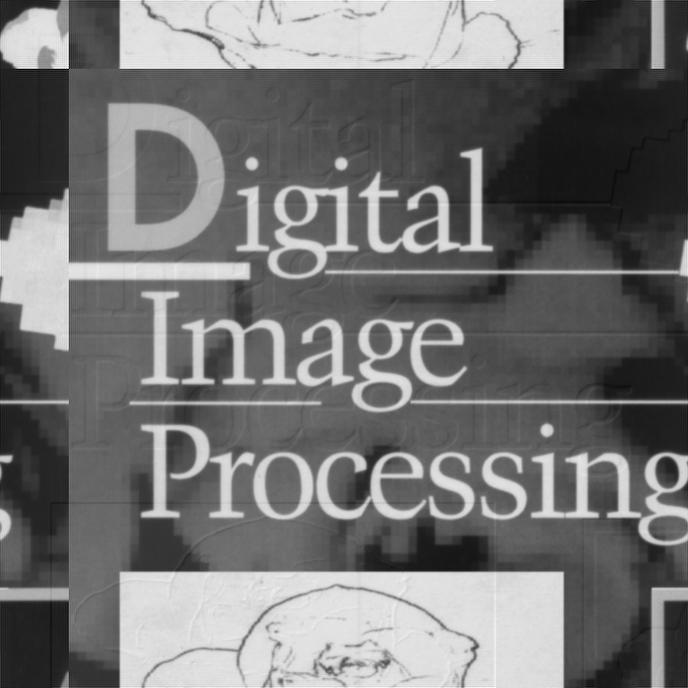
\includegraphics[width=0.25\textwidth] {blurred.jpg}
 }
  ~
 \subfigure[Blurred image with gaussian noise]{
   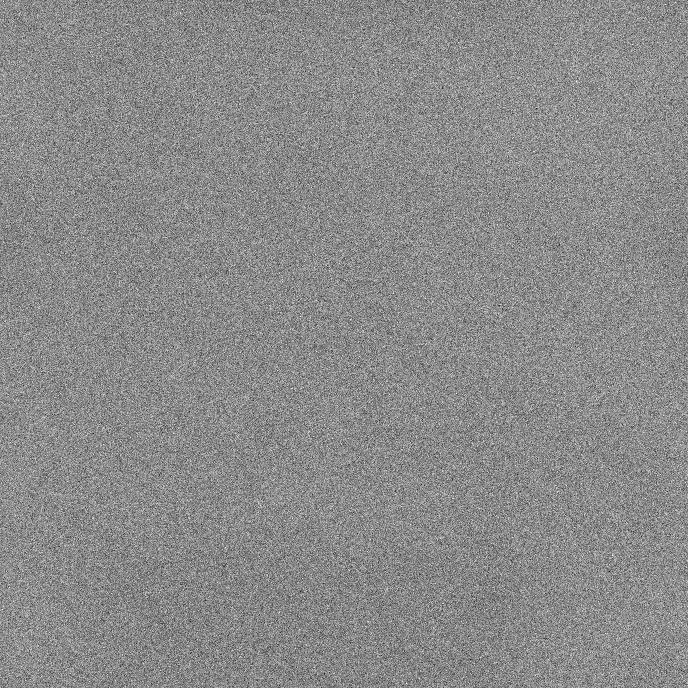
\includegraphics[width=0.25\textwidth] {blurred_w_gauss.jpg}
   \label{fig:subfig1}
 }
 ~
  \subfigure[Inverse Filter]{
   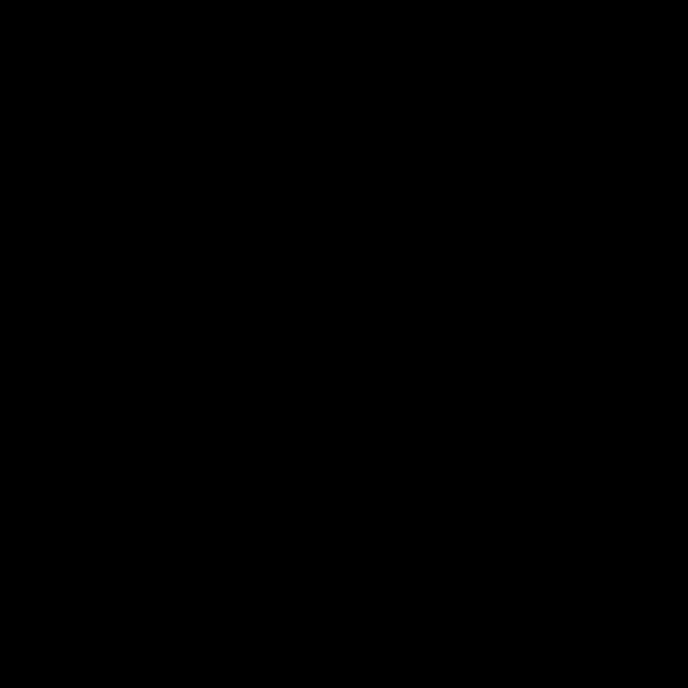
\includegraphics[width=0.25\textwidth] {restored_inversefilt.jpg}
   \label{fig:subfig1}
 }

 \subfigure[Wiener with parameter $k = 2$, power spectrum $p=5$]{
   \includegraphics[width=0.25\textwidth] {restored_wiener_param2-5.jpg}
   \label{fig:subfig1}
 }
 ~
  \subfigure[Wiener with parameter $k = 0.1$, power spectrum $p=1$]{
   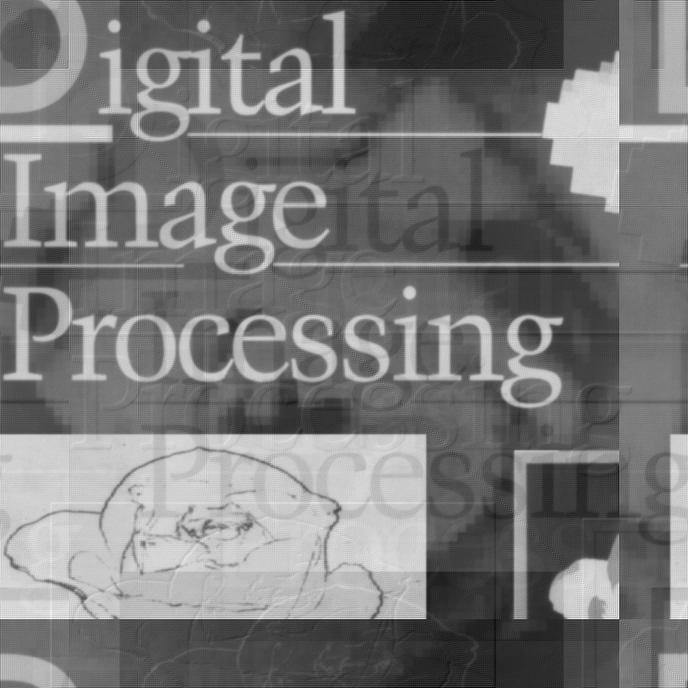
\includegraphics[width=0.25\textwidth] {restored_wiener_param011.jpg}
   \label{fig:subfig1}
 }
 ~
  \subfigure[Wiener with parameter $k = 2$, power spectrum $p=1$]{
   \includegraphics[width=0.25\textwidth] {restored_wiener_param2-1.jpg}
   \label{fig:subfig1}
 }
 ~
  \subfigure[Wiener with parameter $k = 0$, power spectrum $p=5$]{
   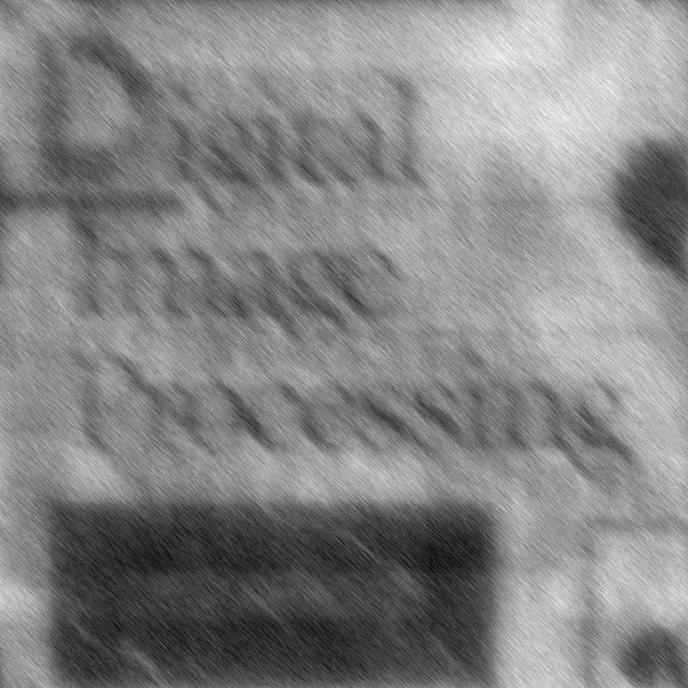
\includegraphics[width=0.25\textwidth] {restored_wiener_param05.jpg}
   \label{fig:subfig1}
 }
  ~
  \subfigure[Wiener with parameter $k = 2$, power spectrum $p=6$]{
   \includegraphics[width=0.25\textwidth] {restored_wiener_param2-6.jpg}
   \label{fig:subfig1}
 }
 
\end{figure*}



\section{Assignment 6}

Using the bilinear and nearest neighbour interpolation methods, we achieve different results for the given operations. 
Generally it can be seen that bilinear interpolation does perform for the given image slightly better, especially when using rotation.
When using translation and scaling, the differences between the two methods are not easily seen. The implementations for scaling and translating are both straightforward and result for both methods in a roughly equal picture.

Bilinear interpolation is given as:
\begin{gather*} 
\begin{array}{ l l}
f(x,y) \approx & \, \frac{f(Q_{11})}{(x_2-x_1)(y_2-y_1)} (x_2-x)(y_2-y) \, + \\
               & \, \frac{f(Q_{21})}{(x_2-x_1)(y_2-y_1)} (x-x_1)(y_2-y) \, + \\
               & \, \frac{f(Q_{12})}{(x_2-x_1)(y_2-y_1)} (x_2-x)(y-y_1) \, + \\
               & \, \frac{f(Q_{22})}{(x_2-x_1)(y_2-y_1)} (x-x_1)(y-y_1) \\
   \qquad          = & \, \frac{1}{(x_2-x_1)(y_2-y_1)} \Big(   f(Q_{11})(x_2-x)(y_2-y) \, + \\
               & \, \qquad \qquad \qquad \qquad \; \;    f(Q_{21})(x-x_1)(y_2-y) \, + \\
               & \, \qquad \qquad \qquad \qquad \; \;    f(Q_{12})(x_2-x)(y-y_1) \, + \\
               & \, \qquad \qquad \qquad \qquad \; \;    f(Q_{22})(x-x_1)(y-y_1) \quad \Big)
\end{array}
\end{gather*}

The rotation was done using the following function:
\begin{minted}[mathescape,
               linenos,
               numbersep=5pt,
               frame=lines,
               framesep=2mm]{python}
def rotate(x, y, theta, ox, oy):
    """Rotate arrays of coordinates x and y by theta radians about the
    point (ox, oy).
    """
    s, c = np.sin(theta), np.cos(theta)
    x, y = np.asarray(x) - ox, np.asarray(y) - oy
    return x * c - y * s + ox, x * s + y * c + oy
\end{minted}


Nearest neightbor interpolation is straight forward:

\begin{minted}[mathescape,
               linenos,
               numbersep=5pt,
               frame=lines,
               framesep=2mm]{python}
def _interpolate(self, sx, sy):
    return np.round(sx).astype(int), np.round(sy).astype(int)

\end{minted}

Bilinear interpolation is somewhat more complex, the formula used to calculate a new point is:

\begin{minted}[mathescape,
               linenos,
               numbersep=5pt,
               frame=lines,
               framesep=2mm]{python}
def _interpolate(self, im, x, y):
        x = np.asarray(x)
        y = np.asarray(y)
    
        x0 = np.floor(x).astype(int)
        x1 = x0 + 1
        y0 = np.floor(y).astype(int)
        y1 = y0 + 1
#         Clip the x0 and x1, so that we dont have to check later if they are in range of the img
        x0 = np.clip(x0, 0, im.shape[1] - 1);
        x1 = np.clip(x1, 0, im.shape[1] - 1);
        y0 = np.clip(y0, 0, im.shape[0] - 1);
        y1 = np.clip(y1, 0, im.shape[0] - 1);
        Ia = im[ y0, x0 ]
        Ib = im[ y1, x0 ]
        Ic = im[ y0, x1 ]
        Id = im[ y1, x1 ]
        wa = (x1 - x) * (y1 - y)
        wb = (x1 - x) * (y - y0)
        wc = (x - x0) * (y1 - y)
        wd = (x - x0) * (y - y0)
        
        return (wa * Ia + wb * Ib + wc * Ic + wd * Id)
\end{minted}





\section{Assignment 7}

\subsection{Standard compression}
The image compression was achieved using four different kernels:
\begin{minted}[mathescape,
               linenos,
               numbersep=5pt,
               frame=lines,
               framesep=2mm]{python}
zonal = np.array([
    [1, 1, 1, 1, 1, 0, 0, 0],
    [1, 1, 1, 1, 0, 0, 0, 0],
    [1, 1, 1, 0, 0, 0, 0, 0],
    [1, 1, 0, 0, 0, 0, 0, 0],
    [1, 0, 0, 0, 0, 0, 0, 0],
    [0, 0, 0, 0, 0, 0, 0, 0],
    [0, 0, 0, 0, 0, 0, 0, 0],
    [0, 0, 0, 0, 0, 0, 0, 0]
])
zonal_best = np.array([
    [1, 1, 1, 1, 1, 1, 1, 0],
    [1, 1, 1, 1, 1, 1, 0, 0],
    [1, 1, 1, 1, 1, 0, 0, 0],
    [1, 1, 1, 1, 0, 0, 0, 0],
    [1, 1, 1, 0, 0, 0, 0, 0],
    [1, 1, 0, 0, 0, 0, 0, 0],
    [1, 0, 0, 0, 0, 0, 0, 0],
    [0, 0, 0, 0, 0, 0, 0, 0]
])
thresholdmask = np.array([
    [1, 1, 0, 1, 0, 0, 0, 0],
    [1, 1, 1, 0, 0, 0, 0, 0],
    [1, 1, 0, 0, 0, 0, 0, 0],
    [1, 0, 0, 0, 0, 0, 0, 0],
    [0, 0, 0, 0, 0, 0, 0, 0],
    [0, 1, 0, 0, 0, 0, 0, 0],
    [0, 0, 0, 0, 0, 0, 0, 0],
    [0, 0, 0, 0, 0, 0, 0, 0]
])
jpegstd = np.array([[16, 11, 10, 16, 24, 40, 51, 61],
                    [12, 12, 14, 19, 26, 58, 60, 55],
                    [14, 13, 16, 24, 40, 57, 69, 56],
                    [14, 17, 22, 29, 51, 87, 80, 62],
                    [18, 22, 37, 56, 68, 109, 103, 77],
                    [24, 35, 55, 64, 81, 104, 113, 92],
                    [49, 64, 78, 87, 103, 121, 120, 101],
                    [72, 92, 95, 98, 112, 100, 103, 99]
                    ])
\end{minted}

Each of the kernels can be used within the program, using a different parameter given in the parameter "-quantmattype". The results for every of these masks can be seen in the Assignment7 directory.

\begin{figure*}[h!]
    \centering
  \subfigure[Rotation by 40 degrees, Nearest neighbour]{
   \includegraphics[width=0.25\textwidth] {rotatedimg_40_nn.jpg}
   \label{fig:subfig1}
 }
 ~
  \subfigure[Rotation by 40 degrees, Bilinear]{
   \includegraphics[width=0.25\textwidth] {rotatedimg_40_bi.jpg}
   \label{fig:subfig1}
 }
 
 
 \subfigure[Rotation by 60 degrees, Nearest neighbour]{
   \includegraphics[width=0.25\textwidth] {rotatedimg_60_nn.jpg}
   \label{fig:subfig1}
 }
 ~
 \subfigure[Rotation by 60 degrees, Bilinear]{
   \includegraphics[width=0.25\textwidth] {rotatedimg_60_bi.jpg}
   \label{fig:subfig1}
 }
 
  \subfigure[Translation by 50, 20 pixels, nearest neighbour]{
   \includegraphics[width=0.25\textwidth] {tranlatedimg_50_20_nn.jpg}
   \label{fig:subfig1}
 }
 ~
  \subfigure[Translation by 50, 20 pixels, bilinear]{
   \includegraphics[width=0.25\textwidth] {tranlatedimg_50_20_bi.jpg}
   \label{fig:subfig1}
 }
 
  \subfigure[Scaled by factor 2, Nearest neighbor]{
   \includegraphics[width=0.25\textwidth] {scaledimg_2_nn.jpg}
   \label{fig:subfig1}
 }
 ~
  \subfigure[Scaled by factor 2, bilinear]{
   \includegraphics[width=0.25\textwidth] {scaledimg_2_bi.jpg}
   \label{fig:subfig1}
 }
\end{figure*}




\subsection{Wavelets}

The wavelets were approached in a totally different scheme than the proposed one by the book. We used purely matrix operations to achieve our goal.

A wavelet transform of an image $A$ can be displayed by:
\begin{gather*}
B = H^T A H
\end{gather*}
where $H$ is the wavelet transform matrix and $B$ is the resulting encoded image.

Constructing $H$ is a little bit complicated. Generally we construct $H$ as having two components. The upper component, which values all sum up to $2$ and the lower component, which sums up to $0$. Therefore we split the matrix $H$ from the beginning on in two halves and then insert the values for the corresponding wavelet.
In the case of Haar wavelets, we used the Kronecker Product:

\begin{gather}
I \otimes h_0 = \left( \begin{array}{ccccccc}
\frac{1}{\sqrt(2)} & \frac{1}{\sqrt(2)} & 0 & 0 & 0 & \ldots & 0 \\
0 & 0 & \frac{1}{\sqrt(2)} & \frac{1}{\sqrt(2)} & 0 & \ldots & 0 \\
0 & 0 & 0 & 0 & \ddots & \ddots & 0 \\
\vdots & \vdots & \vdots & \vdots & \vdots & \ddots & 0\\
0 & 0 & 0 & 0 & 0 & \frac{1}{\sqrt(2)} & \frac{1}{\sqrt(2)}
\end{array} \right)
\end{gather}
\begin{gather}
I \otimes h_1 = \left( \begin{array}{ccccccc}
\frac{1}{\sqrt(2)} & -\frac{1}{\sqrt(2)} & 0 & 0 & 0 & \ldots & 0 \\
0 & 0 & \frac{1}{\sqrt(2)} & -\frac{1}{\sqrt(2)} & 0 & \ldots & 0 \\
0 & 0 & 0 & 0 & \ddots & \ddots & 0 \\
\vdots & \vdots & \vdots & \vdots & \vdots & \ddots & 0\\
0 & 0 & 0 & 0 & 0 & \frac{1}{\sqrt(2)} & -\frac{1}{\sqrt(2)}
\end{array} \right)
\end{gather}
Afterwards we simply concatenate both halves together ( stack them on each other, row wise ) and obtain the transformation matrix $H$.

Calculating the reconstruction is a simple task due to this operation:
\begin{gather*}
A = H B H^T
\end{gather*}

A special notice should be given for the larger wavelets. Here Kronecker product does not work, since it would lead to being $H$ of larger dimension than $A$, which therefore would increase the picture size and fill it with mostly zeros.

For the case that the wavelets having a size larger than 2, we do basically the same procedure like for the Haar wavelets, we insert in each upper half the wavelet $h_0$ and in the lower $h_1$. We use hereby a step size of $2$, so we get for example the following matrix ( $a,b,c,d$ are just place holders for an e.g. daubechies 4-tap, the principle is the same for the 8-tap etc.)
\begin{gather*}
H_{up} = \left( \begin{array}{cccccccc}
a & b & c & d & 0 & \hdots  \\
0 & 0 & a & b & c & d & \hdots & 0\\
0 & 0 & 0 & 0 & \ddots & \ddots & \ddots & 0\\
d & 0 & 0 & 0 & \ldots & a & b & c \\
c & d & 0 & 0 & \ldots & 0 & a & b \\
b & c & d & 0 & \ldots & 0 & 0 & a \\
\end{array}
\right) 
\end{gather*}
As it can be seen the array "rolls" within the matrix. Using this we can easily compute the matrix $H$ for the daubechies, symlet and cohen wavelet.

The calculations for the encoding and decoding still remain the same, and the usage of the inverse function $g_0$,$g_1$ are completely avoided, thus having a much more efficient and clean solution for the wavelet problem.

\begin{figure*}[h!]
    \centering
  \subfigure[Zonal, good quality reconstruction]{
   \includegraphics[width=0.25\textwidth] {zonal_best_reconstructed.jpg}
   \label{fig:subfig1}
 }
 ~
  \subfigure[Zonal, good quality, reconstructed]{
   \includegraphics[width=0.25\textwidth] {zonal_best_diff.jpg}
   \label{fig:subfig1}
 }
 
 
 \subfigure[Threshold mask, reconstruction]{
   \includegraphics[width=0.25\textwidth] {threshold_1_reconstructed.jpg}
   \label{fig:subfig1}
 }
 ~
 \subfigure[Threshold mask, diff]{
   \includegraphics[width=0.25\textwidth] {threshold_1_diff.jpg}
   \label{fig:subfig1}
 }
 
  \subfigure[Threshold mask, reconstruction]{
   \includegraphics[width=0.25\textwidth] {threshold_2_reconstructed.jpg}
   \label{fig:subfig1}
 }
 ~
  \subfigure[Threshold mask, diff]{
   \includegraphics[width=0.25\textwidth] {threshold_2_diff.jpg}
   \label{fig:subfig1}
 }
\end{figure*}

\begin{figure*}[h!]
    \centering
  \subfigure[Haar wavelet encoded]{
   \includegraphics[width=0.25\textwidth] {lena_haar_encoded.jpg}
   \label{fig:subfig1}
 }
 ~
  \subfigure[Haar wavelet, reconstructed, removing all components < 5]{
   \includegraphics[width=0.25\textwidth] {lena_haar_reconstructed.jpg}
   \label{fig:subfig1}
 }
 ~
  \subfigure[Haar, diff]{
   \includegraphics[width=0.25\textwidth] {lena_haar_diff.jpg}
   \label{fig:subfig1}
 }
 
 
 \subfigure[Daubechies 8-tap encoded]{
   \includegraphics[width=0.25\textwidth] {lena_daub_encoded.jpg}
   \label{fig:subfig1}
 }
 ~
 \subfigure[Daubechies 8-tap reconstructed]{
   \includegraphics[width=0.25\textwidth] {lena_daub_reconstructed.jpg}
   \label{fig:subfig1}
 }
 ~
  \subfigure[Daubechies 8-tap diff]{
   \includegraphics[width=0.25\textwidth] {lena_daub_diff.jpg}
   \label{fig:subfig1}
 }
 
  \subfigure[Symlet 8-tap encoded]{
   \includegraphics[width=0.25\textwidth] {lena_sym_encoded.jpg}
   \label{fig:subfig1}
 }
 ~
 \subfigure[Stmlet 8-tap reconstructed]{
   \includegraphics[width=0.25\textwidth] {lena_sym_reconstructed.jpg}
   \label{fig:subfig1}
 }
 ~
  \subfigure[Symlet 8-tap diff]{
   \includegraphics[width=0.25\textwidth] {lena_sym_diff.jpg}
   \label{fig:subfig1}
 }
 
 \subfigure[Cohen 8-tap encoded]{
   \includegraphics[width=0.25\textwidth] {lena_cohen_encoded.jpg}
   \label{fig:subfig1}
 }
 ~
 \subfigure[Cohen 8-tap reconstructed]{
   \includegraphics[width=0.25\textwidth] {lena_cohen_reconstructed.jpg}
   \label{fig:subfig1}
 }
 ~
  \subfigure[Cohen 8-tap diff]{
   \includegraphics[width=0.25\textwidth] {lena_cohen_diff.jpg}
   \label{fig:subfig1}
 }
\end{figure*}




\section{Assignment 8}

In assignment 8 we implemented the techniques boundaryextraction,holefilling,erosion,diletation,opening,closing and connected components.

Since erosion and diltation are the conjugate of each other, we simply negated the logic operators in erosion to get diletation.
\begin{minted}[mathescape,
               linenos,
               numbersep=5pt,
               frame=lines,
               framesep=2mm]{python}
def erosion(inputimg, mask):
    maskoffset = len(mask) / 2
    returnimg = np.zeros(inputimg.shape, dtype=bool)
    for i in range(maskoffset, len(inputimg) - maskoffset):
        for j in range(maskoffset, len(inputimg[0]) - maskoffset):
            curmask = inputimg[i - maskoffset:i + maskoffset + 1, j - maskoffset:j + maskoffset + 1] & mask
            if (curmask == mask).all() :
                returnimg[i, j] = 1
    return returnimg               
\end{minted}

Moreover the diletation is computed only changing the values within the returnedimg. Whereas for erosion we start by having a zeroed array, for diletation we start by having a array filled with ones and zero it out.
\begin{minted}[mathescape,
               linenos,
               numbersep=5pt,
               frame=lines,
               framesep=2mm]{python}
def diletation(inputimg, mask):
    maskoffset = len(mask) / 2
    m, n = inputimg.shape
    returnimg = np.ones((m, n), dtype=bool)
    padimg(returnimg, 0)
    for i in range(maskoffset, len(inputimg) - maskoffset):
        for j in range(maskoffset, len(inputimg[0]) - maskoffset):
            structureelement = inputimg[i - maskoffset:i + maskoffset + 1, j - maskoffset:j + maskoffset + 1] & mask
            if (structureelement == mask).all():
                returnimg[i, j] = 0
    return returnimg
\end{minted}

Opening and closing are just combinations of the operations above.

Boundary following and hole filling is done using again the same algorithms of above, yet their runtime is very slow, so it is not recommended to run these by anybody again ( runtime is at least 30 mins ).

\begin{figure*}[h!]
    \centering
  \subfigure[Noisy fingerprint erosion]{
   \includegraphics[width=0.25\textwidth] {noisy_fingerprint_erosion.jpg}
   \label{fig:subfig1}
 }
 ~
  \subfigure[Noisy fingerprint dilation]{
   \includegraphics[width=0.25\textwidth] {noisy_fingerprint_diletation.jpg}
   \label{fig:subfig1}
 }
 ~
  \subfigure[Noisy fingerprint opening]{
   \includegraphics[width=0.25\textwidth] {noisy_fingerprint_opening.jpg}
   \label{fig:subfig1}
 }
 ~
  \subfigure[Noisy fingerprint closing]{
   \includegraphics[width=0.25\textwidth] {noisy_fingerprint_closing.jpg}
   \label{fig:subfig1}
 }
 
\end{figure*}

\begin{figure*}[h!]
    \centering
  \subfigure[Lincoln Boundary extraction]{
   \includegraphics[width=0.25\textwidth] {licoln_from_penny_boundaryextraction.jpg}
   \label{fig:subfig1}
 }
 ~
  \subfigure[Hole filling with 3x3 mask]{
   \includegraphics[width=0.25\textwidth] {region_filling_holesfilled.jpg}
   \label{fig:subfig1}
 } 
\end{figure*}


\section{Assignment 9}

\subsection{Segementation}

\begin{figure*}[h!]
    \centering
  \subfigure[Global thresholding, beginning with datamean and datamean +20]{
   \includegraphics[width=0.25\textwidth] {global.jpg}
   \label{fig:subfig1}
 }
 ~
  \subfigure[Thresholding using Otsu algorithm]{
   \includegraphics[width=0.25\textwidth] {Otsu.jpg}
   \label{fig:subfig1}
 } 
\end{figure*}



\subsection{Edgedetection}

In this exercise, the maar filter, was firstly used to get some sense of how the filter should work. The implemented filter uses a laplacian mask to firstly get the second derivative of the image. Afterwards the filter finds the zero crossings of a pixels neighbourhood.


The canny filter is therefore by far complexer.

The canny filter has the following 4 steps:
\begin{enumerate}
\item Smooth the image by using a Gaussian
\item Calculate the gradient magnitude 
\item Apply non-maximum suppression
\item Apply hysteresis thresholding
\end{enumerate}


The steps are done using some help of pythons numpy library. We begin by calculate the gradient magnitude and angles. $gx,gy$ are the 2 dimensional grids for the $x,y$ components respectively, which are calculated by applying a sobel or prewitt operator on the image.
\begin{minted}[mathescape,
               linenos,
               numbersep=5pt,
               frame=lines,
               framesep=2mm]{python}
def gradientmagnitude(gx, gy):
    return np.hypot(gx,gy)


def directionangle(gx, gy):
    return np.arctan2(gy , gx)
\end{minted}

After the angles and the magnitudes are calculated, we normalize the angles to go in four different directions: $0,45,90,-45$, by simply checking the angle range:
\begin{minted}[mathescape,
               linenos,
               numbersep=5pt,
               frame=lines,
               framesep=2mm]{python}
angle[(angle < 22.5) | (angle > 337.5) & (angle < 202.5) | (angle > 157.5) ] = 0.
angle[((angle >= 22.5) & (angle <= 67.5)) | ((angle >= 202.5) & (angle <= 247.5))] = 45.
angle[((angle > 67.5) & (angle < 112.5)) | ((angle >= 247.5) & (angle <= 292.5))] = 90.
angle[((angle <= 157.5) & (angle > 112.5)) | ((angle >= 292.5) & (angle <= 337.5))] = -45.
\end{minted}

Maximum suppression is achieved by setting specific values in the mag matrix to zero:

\begin{minted}[mathescape,
               linenos,
               numbersep=5pt,
               frame=lines,
               framesep=2mm]{python}
mag_sup = np.copy(mag)
    for x in range(1, width - 1):
        for y in range(1, height - 1):
            if angle[x][y] == 0:
                if (mag[x][y] <= mag[x][y + 1]) or \
                   (mag[x][y] <= mag[x][y - 1]):
                    mag_sup[x][y] = 0
            elif angle[x][y] == 45:
                if (mag[x][y] <= mag[x - 1][y + 1]) or \
                   (mag[x][y] <= mag[x + 1][y - 1]):
                    mag_sup[x][y] = 0
            elif angle[x][y] == 90:
                if (mag[x][y] <= mag[x + 1][y]) or \
                   (mag[x][y] <= mag[x - 1][y]):
                    mag_sup[x][y] = 0
            else:
                if (mag[x][y] <= mag[x + 1][y + 1]) or \
                   (mag[x][y] <= mag[x - 1][y - 1]):
                    mag_sup[x][y] = 0
\end{minted}

Edge linking is the process to link all low-thresholded edges to the high ones, whereas the high edges are the ones which are filtered by a larger threshold than the low ones, e.g.:
\begin{minted}[mathescape,
               linenos,
               numbersep=5pt,
               frame=lines,
               framesep=2mm]{python}
m = np.max(mag_sup)      
th = m*0.1
tl = th/2
gnh = np.zeros((width, height),dtype=float)
    gnl = np.zeros((width, height),dtype=float)
    for x in range(1,width-1):
        for y in range(1,height-1):
            if mag_sup[x][y] >= th:
                gnh[x][ y] = mag_sup[x][y]
            if mag_sup[x][y] >= tl:
                gnl[x][ y] = mag_sup[x][y]
gnl = gnl - gnh
def traverse(i, j):
        x = [-1, 0, 1, -1, 1, -1, 0, 1]
        y = [-1, -1, -1, 0, 0, 1, 1, 1]
        for k in range(8):
            if gnh[i + x[k]][j + y[k]] == 0 and gnl[i + x[k]][j + y[k]] != 0:
                gnh[i + x[k]][j + y[k]] = 1
                traverse(i + x[k], j + y[k])
for i in range(1, width - 1):
        for j in range(1, height - 1):
            if gnh[i][j]:
                gnh[i, j] = 1
                traverse(i, j)
\end{minted}               
After traversing the items, the edge linking is done and the array is returned, which contains the picture of the canny edge detection.


\begin{figure*}[h!]
    \centering
  \subfigure[Roberts edge detector]{
   \includegraphics[width=0.25\textwidth] {roberts.jpg}
   \label{fig:subfig1}
 }
 ~
  \subfigure[Sobel of image]{
   \includegraphics[width=0.25\textwidth] {sobel.jpg}
   \label{fig:subfig1}
 } 
 ~
  \subfigure[Prewitt of image]{
   \includegraphics[width=0.25\textwidth] {prewitt.jpg}
   \label{fig:subfig1}
 } 
 ~
  \subfigure[Maar hidlret of image]{
   \includegraphics[width=0.25\textwidth] {marr_hidlret.jpg}
   \label{fig:subfig1}
 } 
 ~
  \subfigure[Canny edge detector]{
   \includegraphics[width=0.25\textwidth] {canny.jpg}
   \label{fig:subfig1}
 } 
\end{figure*}


\section{Assignment 10}

The last Assignment is about using boundary following to extract chain codes and using PCA for compression.

\subsection{Boundary following}

To follow the boundary we used the following algorithm:
\begin{enumerate}
\item Put first point , marked as $b_0$ in a stack and save it's coordinates.
\item Pop the point in the list, which was added last call it $b$.
\item If that $b$ is the very first popped $b$, save during this iteration the coordinates of the found point as $b_1$, else skip
\item Use $b$ and get the corresponding $c$ and start to iterate in clockwise one full round from $c$ on.
\item If another point is found during that iteration , store it in the iteration list and also save the position of the new point's starting-point 
\item Do it as long as you reach the point $b_1$ again.
\end{enumerate}

In our implementation we use a class to store the objects $b$ and $c$.

\begin{minted}[mathescape,
               linenos,
               numbersep=5pt,
               frame=lines,
               framesep=2mm]{python}
class Point():
    ''' A container for the given Points, stores 2 variables and returns an iterator and a given item
        The iterator returns for the current point the circle around it.
    '''
    neighboriter = zip(xstep, ystep)
    
    def __init__(self, b, c):
        self.b = b
        self.c = c
        
    def __repr__(self):
        ret = "".join(str(self.b))
        return ret
    
    def __iter__(self):
        index = self.neighboriter.index(self.c)
#         We need to check both of the slices, we get on one side the left over circle and on the other, the "togo"
        return iter(self.neighboriter[index:] + self.neighboriter[:index])
    
    def __getitem__(self, key):
        index = self.neighboriter.index(self.c)
        iterlist = self.neighboriter[index:] + self.neighboriter[:index]
        return iterlist[key]
#     During looping, the in operator can be used to check the b value
    def __eq__(self, other):
        return other == self.b
\end{minted}


When calculating the first difference, we used the following formula.
Given two adjacent elements $c_i,c_{i+1} \in C$, when using $b$ different angles ( $b=8$ in our case ), we calculate:
\begin{gather*}
s = (b - ( c_i - c_{i+1} )) \mod b
\end{gather*}
Which gives us the correct results, using the modulo operator as "mod"


\begin{figure*}[h!]
    \centering
  \subfigure[Followed boundary after applying blur on image]{
   \includegraphics[width=0.25\textwidth] {boundary_followed.jpg}
   \label{fig:subfig1}
 }
 ~
  \subfigure[Followed boundary after applying blur on image]{
   \includegraphics[width=0.25\textwidth] {grid.jpg}
   \label{fig:subfig1}
 }
\end{figure*}

The chaincodes can be seen in the file "Chaincode".

\subsection{PCA} 
Principal component analysis (PCA) is a statistical procedure that uses an orthogonal transformation to convert a set of observations of possibly correlated variables into a set of values of linearly uncorrelated variables called principal components. The number of principal components is less than or equal to the number of original variables. This transformation is defined in such a way that the first principal component has the largest possible variance (that is, accounts for as much of the variability in the data as possible), and each succeeding component in turn has the highest variance possible under the constraint that it is orthogonal to (i.e., uncorrelated with) the preceding components. The principal components are orthogonal because they are the eigenvectors of the covariance matrix, which is symmetric. PCA is sensitive to the relative scaling of the original variables.

The results of the PCA compression can be seen in the Assignment 10 folder.

\begin{figure*}[h!]
    \centering
  \subfigure[First PC component]{
   \includegraphics[width=0.25\textwidth] {PC_Component_1.jpg}
   \label{fig:subfig1}
 }
 ~
  \subfigure[Second PC component]{
   \includegraphics[width=0.25\textwidth] {PC_Component_2.jpg}
   \label{fig:subfig1}
 } 
 
  \subfigure[First component reconstructed]{
   \includegraphics[width=0.25\textwidth] {Reconstructed_1.jpg}
   \label{fig:subfig1}
 } 
 ~
  \subfigure[Second component reconstructed]{
   \includegraphics[width=0.25\textwidth] {Reconstructed_2.jpg}
   \label{fig:subfig1}
 } 
 ~
  \subfigure[3rd component reconstructed]{
   \includegraphics[width=0.25\textwidth] {Reconstructed_3.jpg}
   \label{fig:subfig1}
 } 
   \subfigure[4th component reconstructed]{
   \includegraphics[width=0.25\textwidth] {Reconstructed_4.jpg}
   \label{fig:subfig1}
 } 
 ~
  \subfigure[5th component reconstructed]{
   \includegraphics[width=0.25\textwidth] {Reconstructed_5.jpg}
   \label{fig:subfig1}
 } 
   \subfigure[6th component reconstructed]{
   \includegraphics[width=0.25\textwidth] {Reconstructed_6.jpg}
   \label{fig:subfig1}
 } 
 
  \subfigure[Diff 1st component]{
   \includegraphics[width=0.25\textwidth] {Diff_1.jpg}
   \label{fig:subfig1}
 } 
 ~
 \subfigure[Diff 2nd component]{
   \includegraphics[width=0.25\textwidth] {Diff_2.jpg}
   \label{fig:subfig1}
 }
 ~
 \subfigure[Diff 3rd component]{
   \includegraphics[width=0.25\textwidth] {Diff_3.jpg}
   \label{fig:subfig1}
 } 
 ~
 \subfigure[Diff 4th component]{
   \includegraphics[width=0.25\textwidth] {Diff_4.jpg}
   \label{fig:subfig1}
 } 
 ~
 \subfigure[Diff 5th component]{
   \includegraphics[width=0.25\textwidth] {Diff_5.jpg}
   \label{fig:subfig1}
 } 
 ~
 \subfigure[Diff 6th component]{
   \includegraphics[width=0.25\textwidth] {Diff_6.jpg}
   \label{fig:subfig1}
 }  
\end{figure*}